\begin{name}
	{\tenchude}
	{TOÁN 11}
	{LỚP TOÁN THẦY PHÁT}
	{Thời gian: 90 phút - Không kể thời gian phát đề}
\end{name}
\TN
\Opensolutionfile{ans}[ans/ans-1-GK1-KNTT-De15-NH23-24]

%%==========Câu 1
\begin{ex}%[1K1Y1-5] 
	$\sin\alpha>0$ khi điểm cuối của cung $\alpha$ trên đường tròn lượng giác thuộc các góc phần tư thứ
	\choice
	{I và III}
	{\True I và II}
	{II và IV}
	{I và IV}
	\loigiai{
		$\sin\alpha>0$ khi điểm cuối của cung $\alpha$ trên đường tròn lượng giác các góc phần tư thứ I và II.	
	}
\end{ex}
	\begin{ex}%[1K1Y1-8]
	Trong các khẳng định sau, khẳng định nào sai?
	\choice
	{$\tan\left(\pi-\alpha\right)=-\tan\alpha$}
	{\True $\tan\left(\pi+\alpha\right)=-\tan\alpha$}
	{$\tan\left(-\alpha\right)=-\tan\alpha$}
	{$\tan\left(\dfrac{\pi}{2}-\alpha\right)=\cot\alpha$}
	\loigiai{
		Vì $\tan\left(\pi+\alpha\right)=\tan\alpha$ nên khẳng định sai là $\tan\left(\pi+\alpha\right)=-\tan\alpha$.	
	}
\end{ex}

\begin{ex}%[1K1Y2-1]
	Trong các công thức sau, công thức nào đúng?
	\choice
	{\True $\sin\left(a-b\right)=\sin a\cdot\cos b-\sin b\cdot\cos a$}
	{$\cos\left(a-b\right)=\cos a\cdot\cos b-\sin a\cdot\sin b$}
	{$\sin\left(a+b\right)=\sin a\cdot\cos b-\sin b\cdot\cos a$}
	{$\cos\left(a+b\right)=\cos a\cdot\cos b$ $+$ $\sin a\cdot\sin b$}
	\loigiai{
		Công thức cộng $\sin\left(a-b\right)=\sin a\cdot\cos b-\sin b\cdot\cos a$.	
	}
\end{ex}
\begin{ex}%[1K1K2-1]
	Rút gọn biểu thức $\sin\left(a-17^\circ\right)\cos\left(a+13^\circ\right)-\sin\left(a+13^\circ\right)\cos\left(a-17^\circ\right)$, ta được
\choice
{$\sin2a$}
{$\cos2a$}
{\True $-\dfrac{1}{2}$}
{$\dfrac{1}{2}$}
\loigiai{ 
	Ta có $\sin\left(a-17^\circ\right)\cdot\cos\left(a+13^\circ\right)-\sin\left(a+13^\circ\right)\cdot\cos\left(a-17^\circ\right)=\sin\left[\left(a-17^\circ\right)-\left(a+13^\circ\right)\right]$\\
	$=\sin\left(-30^\circ\right)=-\dfrac{1}{2}$.	
	}
\end{ex}
\begin{ex}%[1K1Y3-4]
	Hàm số $y=\sin x$ tuần hoàn với chu kỳ là 
	\choice
	{$\dfrac{\pi}{2}$}
	{$\dfrac{\pi}{3}$}
	{\True $2\pi$}
	{$\pi$}
	\loigiai{
		Hàm số $y=\sin x$ tuần hoàn với chu kỳ là $2\pi$.
	}
\end{ex}
\begin{ex}%[1K1B3-1]
	Tìm tập xác định $\mathscr{D}$ của hàm số $y=\dfrac{3\tan x-5}{1-\sin^2 x}$.
	\choice
	{$\mathscr{D}=\mathbb{R}\setminus\left\{\dfrac{\pi}{2}+k2\pi,k\in\mathbb{Z}\right\}$}
	{\True $\mathscr{D}=\mathbb{R}\setminus\left\{\dfrac{\pi}{2}+k\pi,k\in\mathbb{Z}\right\}$}
	{$\mathscr{D}=\mathbb{R}\setminus\left\{\pi+k\pi,k\in\mathbb{Z}\right\}$}
	{$\mathscr{D}=\mathbb{R}$}
	\loigiai{
	Hàm số xác định khi và chỉ khi $\heva{&1-\sin^2 x\neq 0\\&\cos x\neq 0}$\\
	$\Leftrightarrow \heva{&\sin^2 x\neq 1\\&\cos x\neq 0} \Leftrightarrow \cos x\neq 0 \Leftrightarrow x\neq\dfrac{\pi}{2}+k\pi,k\in\mathbb{Z}$.\\
	Vậy tập xác định của hàm số là $\mathscr{D}=\mathbb{R}\setminus\left\{\dfrac{\pi}{2}+k\pi,k\in\mathbb{Z}\right\}$. 
	}
\end{ex}

\begin{ex}%[Dự án 1 - TLDH - TeamTeXHoa - Sauluoi3105]%[1K2B5-4]
	Trong các dãy số $\left(u_n\right)$ sau đây, dãy số nào là dãy số bị chặn?
	\choice
	{$u_n=\sqrt{n^2+1}$}
	{$u_n=n+\dfrac{1}{n}$}
	{$u_n=2^n+1$}
	{\True $u_n=\dfrac{n}{n+1}$}
	\loigiai{
		Ta có $0<u_n=\dfrac{n}{n+1}=1-\dfrac{1}{n+1}<1,\,\forall n \in \mathbb{N^*}$.\\
		Suy ra dãy số $u_n=\dfrac{n}{n+1}$ bị chặn.
	}
\end{ex}

\begin{ex}%[1K2B6-3]
	Cho cấp số cộng $\left(u_{n}\right)$ với $u_{1}=-2$ và công sai $d=3$ thì số hạng $u_{5}$ bằng
	\choice
	{$7$}
	{\True $10$}
	{$5$}
	{$6$}
	\loigiai{
		Áp dụng công thức số hạng thứ $n$ của cấp số cộng $\left(u_{n}\right)$ là $u_{n}=u_{1}+\left(n-1\right)\cdot d$.\\
		Khi đó số hạng $u_{5}=u_{1}+\left(5-1\right)\cdot d=-2+4\cdot3=10$. Vậy $u_{5}=10$.	
	}
\end{ex}

\begin{ex}%[1K2K7-1]
	Cho cấp số nhân $\left(u_{n}\right)$ có công bội dương và $u_{2}=\dfrac{1}{5}$, $u_{4}=5$. Tính công bội $q$.
	\choice
	{\True $5$}
	{$25$}
	{$\dfrac{1}{5}$}
	{$125$}
	\loigiai{
		Ta có $\heva{&u_{2}=u_{1}\cdot q=\dfrac{1}{5}\\&u_{4}=u_{1}\cdot q^3=5} \Rightarrow \dfrac{u_{4}}{u_{2}}=q^2=25 \Leftrightarrow q=\pm5$.\\
		Mà cấp số nhân $\left(u_{n}\right)$ có công bội dương nên $q=5$.
	}
\end{ex}

\begin{ex}%[1K3Y8-1]
	Mẫu số liệu sau cho biết phân bố theo độ tuổi của dân số Việt Nam năm $2019$\\
	\begin{center}
		\begin{tabular}{|c|c|c|c|}
		\hline
		Độ tuổi& Dưới $15$ & Từ $15$ đến $65$ & Từ $65$ trở lên\\
		\hline
		Số người& $23 371 882$ & $65 420 451$ & $7 416 651$\\
		\hline
	\end{tabular}
	\end{center}
	Số dân Việt Nam năm $2019$ là
	\choice
	{$73837102$}
	{$72837102$}
	{$95208984$}
	{\True $96208984$}
	\loigiai{
		Số dân Việt Nam năm $2019$ là $23371882+65420451+7416651= 96208984$.	
	}
\end{ex}
\begin{ex}%[1K3Y9-4]
	Khảo sát thời gian tập thể dục của một số học sinh khối $11$ thu được mẫu số liệu ghép nhóm sau
	\begin{center}
		\begin{tabular}{|c|c|c|c|c|c|}
			\hline
			Thời gian $\left(\text{phút}\right)$& $\left[0;20\right)$ & $\left[20;40\right)$ & $\left[40;60\right)$& $\left[60;80\right)$ & $\left[80;100\right)$\\
			\hline
			Số học sinh & $5$ & $9$ & $12$ & $10$ & $6$\\
			\hline
		\end{tabular}
	\end{center}
	Nhóm chứa mốt của mẫu số liệu trên là
	\choice
	{$\left[20;40\right)$}
	{$\left[60;80\right)$}
	{\True $\left[40;60\right)$}
	{$\left[80;100\right)$}
	\loigiai{
		Mốt $M_0$ chứa trong nhóm $\left[40;60\right)$.		
	}
\end{ex}
\begin{ex}%[1K3K9-3]
	Khảo sát thời gian tập thể dục của một số học sinh khối $11$ thu được mẫu số liệu ghép nhóm sau
	\begin{center}
		\begin{tabular}{|c|c|c|c|c|c|}
			\hline
			Thời gian $\left(\text{phút}\right)$& $\left[0;20\right)$ & $\left[20;40\right)$ & $\left[40;60\right)$& $\left[60;80\right)$ & $\left[80;100\right)$\\
			\hline
			Số học sinh & $5$ & $9$ & $12$ & $10$ & $6$\\
			\hline
		\end{tabular}
	\end{center}
	Nhóm chứa tứ phân vị thứ ba của mẫu số liệu trên là
	\choice
	{$\left[20;40\right)$}
	{\True $\left[60;80\right)$}
	{$\left[40;60\right)$}
	{$\left[80;100\right)$}
	\loigiai{
		Ta có $n=42$ nên tứ phân vị thứ ba của mẫu số liệu trên là $Q_3=x_{33}$.\\
		Mà $x_{33}\in\left[60;80\right)$.\\
		Vậy nhóm chứa tứ phân vị thứ ba của mẫu số liệu trên là nhóm $\left[60;80\right)$.		
	}
\end{ex}

\TNTF
\begin{ex}%[Thống kê – Trung bình và tứ phân vị]
Một cửa hàng đồng hồ khảo sát số tiền (triệu đồng) mà khách hàng sẵn sàng chi cho một chiếc đồng hồ cao cấp. Kết quả được cho như sau:
\begin{center}
\begin{tabular}{|c|c|c|c|c|}
\hline
Mức giá & $[10;15)$ & $[15;20)$ & $[20;25)$ & $[25;30)$ \\
\hline
Số khách hàng & $22$ & $58$ & $40$ & $20$ \\
\hline
\end{tabular}
\end{center}
\choiceTF
{\True Cỡ mẫu là $140$}
{\True Trung bình cộng khoảng $20{,}1$}
{$Q_1 \approx 16{,}7$}
{\True $Q_3 \approx 23{,}1$}
\loigiai{
	\begin{itemchoice}
		\itemch Cỡ mẫu: $n = 22 + 58 + 40 + 20 = 140$.
		\itemch Giá trị đại diện: $12{,}5; 17{,}5; 22{,}5; 27{,}5$.\\
		$\overline{x} = \dfrac{12{,}5 \cdot 22 + 17{,}5 \cdot 58 + 22{,}5 \cdot 40 + 27{,}5 \cdot 20}{140} \approx 20{,}1$.
		\itemch $Q_1$: $\dfrac{n}{4} = 35$. Nhóm $[15;20)$ chứa $Q_1$.\\
		$Q_1 = 15 + \dfrac{35 - 22}{58} \cdot 5 \approx 16{,}7$.
		\itemch $Q_3$: $\dfrac{3n}{4} = 105$. Nhóm $[20;25)$ chứa $Q_3$.\\
		$Q_3 = 20 + \dfrac{105 - 80}{40} \cdot 5 \approx 23{,}1$.
	\end{itemchoice}
}
\end{ex}
\begin{ex}%[1D2V3-6]
Cho dãy số $\left(u_n\right)$, biết $\heva{
& u_1=3 \\
& u_{n+1}=4u_n-1}$ (với $\left( n \in \mathbb{N}^*\right)$. Xét tính đúng sai của các khẳng định sau
\choiceTF[t]
{Số hạng thứ năm của dãy số là $685$}
{\True Đặt $v_n=u_n-\dfrac{1}{3}$ thì $\left(v_n\right)$ là cấp số nhân}
{\True Số hạng tổng quát $u_n=\dfrac{8}{3} \cdot 4^{n-1}+\dfrac{1}{3}$}
{\True $S_8=58\,256$}
\loigiai{
\begin{itemchoice}
\itemch  \textbf{Sai.}\\
Ta có $u_2=4u_1-1=4\cdot3-1=12-1=11$; $u_3=4u_2-1=4 \cdot 11-1=44-1=43$\\
$u_4=4u_3-1=4 \cdot 43-1=172-1=171$; $u_5=4u_4-1=4 \cdot 171-1=684-1=683$.\\
Vậy số hạng thứ năm của dãy số là $u_5=683$.
\itemch  \textbf{Đúng.}\\
Ta có $u_{n+1}=4u_n-1 \Leftrightarrow u_{n+1}-\dfrac{1}{3}=4\left(u_n-\dfrac{1}{3}\right)$.\\
Đặt $v_n=u_n-\dfrac{1}{3}$. Ta có $v_{n+1}=4v_n$. Suy ra $\left(v_n\right)$ là cấp số nhân.
\itemch  \textbf{Đúng.}\\
Ta có $v_{n+1}=4v_n$. Suy ra $\left(v_n\right)$ là cấp số nhân với $\heva{
& q=4 \\
& v_1=u_1-\dfrac{1}{3}=\dfrac{8}{3}.}$\\
Suy ra $v_n=v_1 \cdot q^{n-1}=\dfrac{8}{3} \cdot 4^{n-1} \Rightarrow u_n=\dfrac{8}{3} \cdot 4^{n-1}+\dfrac{1}{3}$.
\itemch  \textbf{Đúng.}\\
Ta có $S_8=u_1+u_2+\ldots+u_8=\dfrac{8}{3} \cdot\left(1+4+4^2+\ldots+4^7\right)+\dfrac{1}{3} \cdot 8=58\,256$.
\end{itemchoice}
}
\end{ex}

\TNSA
\begin{ex}%[1K1K3-5]
	Biết hàm số $y=\sqrt{3}\sin 2x - \cos 2x -1$ có tập giá trị là $[m;M]$. Giá trị của $M+m$ bằng 
	\shortans{-2}
	\loigiai{
		Ta có $y=\sqrt{3}\sin 2x - \cos 2x -1=2\left(\dfrac{\sqrt{3}}{2}\sin 2x -\dfrac{1}{2}\cos 2x\right)-1= 2\sin\left(2x-\dfrac{\pi}{6}\right)-1$\\
		Vì $\forall x\in\mathbb{R}, -1\leq \sin\left(2x-\dfrac{\pi}{6}\right)\leq1$ nên suy ra $-2 -1\leq 2\sin\left(2x-\dfrac{\pi}{6}\right)-1\leq2-1$.\\
		Do đó, $-3\leq y\leq1,\forall x\in\mathbb{R}$.\\
		Do đó giá trị lớn nhất và giá trị nhỏ nhất của hàm số $y=\sqrt{3}\sin 2x - \cos 2x -1$ lần lượt là $M=1,m=-3$.\\
		Khi $\sin\left(2x-\dfrac{\pi}{6}\right)=1 \Leftrightarrow 2x-\dfrac{\pi}{6}=\dfrac{\pi}{2}+k2\pi \Leftrightarrow x=\dfrac{\pi}{3}+k2\pi,k\in\mathbb{Z}$.\\
		$\sin\left(2x-\dfrac{\pi}{6}\right)=-1 \Leftrightarrow 2x-\dfrac{\pi}{6}=-\dfrac{\pi}{2}+k2\pi \Leftrightarrow x=-\dfrac{\pi}{6}+k\pi,k\in\mathbb{Z}$.\\
		Vậy $M+m=1-3=-2$.
	}
\end{ex}

\begin{ex}%[1K1K4-5]
	Tổng tất cả các nghiệm của phương trình $\sin\left(x+\dfrac{\pi}{4}\right)+\cos\left(x-\dfrac{3\pi}{4}\right)=0$ thuộc $\left(0;5\pi\right)$ bao nhiêu? (làm tròn đến hàng phần chục)
	\shortans{31,4}
	\loigiai{
		Ta có\\
		$\sin\left(x+\dfrac{\pi}{4}\right)+\cos\left(x-\dfrac{3\pi}{4}\right)=0 \Leftrightarrow \sin x\cdot\cos\dfrac{\pi}{4}+\cos x\cdot\sin\dfrac{\pi}{4}+\cos x\cdot\cos\dfrac{3\pi}{4}+\sin x\cdot\sin\dfrac{3\pi}{4}=0$\\
		$\Leftrightarrow \sqrt{2}\sin x=0 \Leftrightarrow \sin x=0 \Leftrightarrow x=k\pi,k\in\mathbb{Z}$.\\
		Vì $x\in\left(0;5\pi\right) \Rightarrow 0<k\pi<5\pi \Leftrightarrow 0<k<5$.\\
		Vì $k\in\mathbb{Z} \Rightarrow k\in\left\{1;2;3;4\right\} \Rightarrow x\in\left\{\pi;2\pi;3\pi;4\pi\right\}$.\\
		Khi đó, tổng các nghiệm của phương trình là $S=\pi+2\pi+3\pi+4\pi=10\pi$.	
	}
\end{ex}
\begin{ex}%[1K2G6-6]
	Vào năm $2023$, nhiệt độ trung bình của thành phố $A$ là khoảng $29{,}5^\circ C$. Giả sử do biến đổi khí hậu nên mỗi năm nhiệt độ trung bình của thành phố $A$ đều tăng thêm khoảng $0{,}1^\circ C$. Hãy ước tính kể từ năm nào thì nhiệt độ trung bình của thành phố $A$ đạt từ $35^\circ C$ trở lên.
	\shortans{2078}
	\loigiai{
		Theo bài toán, nhiệt độ trung bình ở mỗi năm của thành phố $A$ lập thành cấp số cộng với công sai là $d=0{,}1\left(^\circ C\right)$ và $u_{1}=29{,}5^\circ C$ là nhiệt độ trung bình của thành phố $A$ vào năm $2023$.\\
		Giả sử số hạng thứ $n$ của cấp số cộng có giá trị lớn hơn hoặc bằng $35$.\\
		Tức là, $u_{n}\geq35^\circ C$ hay $u_{1}+\left(n-1\right)\cdot d\geq35 \Leftrightarrow 29{,}5+\left(n-1\right)\cdot0{,}1\geq35 \Leftrightarrow n\geq56$.\\
		Do đó, kể từ số hạng thứ $56$ trở đi thì chúng đều có giá trị lớn hơn hoặc bằng $35$.\\
		Ta có $u_{1}$ là nhiệt độ trung bình của thành phố $A$ vào năm $2023$.\\
		Nên $u_{56}$ là nhiệt độ trung bình của thành phố $A$ vào năm $\left(2023+56-1\right)=2078$.\\
		Vậy kể từ năm $2078$ thì nhiệt độ trung bình của thành phố $A$ đạt từ $35^\circ C$ trở lên. 	
	}
\end{ex}

\begin{ex}%[1D2V1-6]
Với mỗi số nguyên dương $n$, lấy $n+6$ điểm cách đều nhau trên đường tròn. Nối mỗi điểm với điểm cách nó hai điểm trên đường tròn đó để tạo thành các ngôi sao như dưới.
\begin{center}
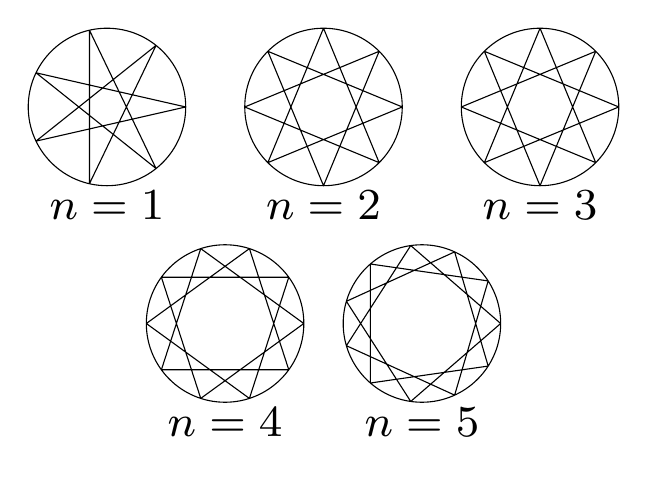
\begin{tikzpicture}[line join = round, line cap=round,>=stealth,font=\footnotesize,scale=.5]

\begin{scope}[xshift=-2cm]
\pgfmathsetmacro{\n}{360/7}
\def\r{2}
\draw
(0,0) circle(\r cm)
(\n*5:\r)--(\n:\r)--(\n*4:\r)
(\n*6:\r)--(\n*2:\r)--(\n*5:\r)
(\n*7:\r)--(\n*3:\r)--(\n*6:\r)
(\n*8:\r)--(\n*4:\r)--(\n*7:\r);
\draw (0,-2.5) node[scale=2]{$n=1$};
\end{scope}

\begin{scope}[xshift=3.5cm]
\pgfmathsetmacro{\n}{360/8}
\def\r{2}
\draw
(0,0) circle(\r cm)
(\n*6:\r)--(\n:\r)--(\n*4:\r)
(\n*7:\r)--(\n*2:\r)--(\n*5:\r)
(\n*8:\r)--(\n*3:\r)--(\n*6:\r)
(\n*9:\r)--(\n*4:\r)--(\n*7:\r)
(\n*10:\r)--(\n*5:\r)--(\n*8:\r);
\draw (0,-2.5) node[scale=2]{$n=2$};
\end{scope}

\begin{scope}[xshift=9cm]
\pgfmathsetmacro{\n}{360/8}
\def\r{2}
\draw
(0,0) circle(\r cm)
(\n*6:\r)--(\n:\r)--(\n*4:\r)
(\n*7:\r)--(\n*2:\r)--(\n*5:\r)
(\n*8:\r)--(\n*3:\r)--(\n*6:\r)
(\n*9:\r)--(\n*4:\r)--(\n*7:\r)
(\n*10:\r)--(\n*5:\r)--(\n*8:\r);
\draw (0,-2.5) node[scale=2]{$n=3$};
\end{scope}

\begin{scope}[xshift=1cm,yshift=-5.5cm]
\pgfmathsetmacro{\n}{360/10}
\def\r{2}
\draw
(0,0) circle(\r cm)
(\n*4:\r)--(\n:\r)--(\n*8:\r)
(\n*5:\r)--(\n*2:\r)--(\n*9:\r)
(\n*6:\r)--(\n*3:\r)--(\n*10:\r)
(\n*7:\r)--(\n*4:\r)--(\n*11:\r)
(\n*8:\r)--(\n*5:\r)--(\n*12:\r)
(\n*9:\r)--(\n*6:\r)--(\n*13:\r)
(\n*10:\r)--(\n*7:\r)--(\n*14:\r)
;
\draw (0,-2.5) node[scale=2]{$n=4$};
\end{scope}

\begin{scope}[xshift=6cm,yshift=-5.5cm]
\pgfmathsetmacro{\n}{360/11}
\def\r{2}
\draw
(0,0) circle(\r cm)
(\n*4:\r)--(\n:\r)--(\n*9:\r)
(\n*5:\r)--(\n*2:\r)--(\n*10:\r)
(\n*6:\r)--(\n*3:\r)--(\n*11:\r)
(\n*7:\r)--(\n*4:\r)--(\n*12:\r)
(\n*8:\r)--(\n*5:\r)--(\n*13:\r)
(\n*9:\r)--(\n*6:\r)--(\n*14:\r)
(\n*10:\r)--(\n*7:\r)--(\n*15:\r)
(\n*11:\r)--(\n*8:\r)--(\n*16:\r)
;
\draw (0,-2.5) node[scale=2]{$n=5$};
\end{scope}

\end{tikzpicture}
\end{center}

Gọi $u_n$ là số đo góc ở đỉnh tính theo đơn vị độ của mỗi ngôi sao thì ta được dãy số $\left(u_n\right)$. Tính $u_6$.
\shortans[oly]{$90$}
\loigiai{
Ta thấy đường tròn được chia thành $n+6$ cung bằng nhau và mỗi cung có số đo bằng $\left(\dfrac{360}{n+6}\right)^\circ$.\\
Do mỗi điểm được nối với điểm cách nó hai điểm trên đường tròn nên góc ở đỉnh của mỗi ngôi sao là góc nội tiếp chắn $n+6-2\cdot3=n$ cung bằng nhau đó.\\
Suy ra số đo góc ở đỉnh tính theo đơn vị độ của mỗi ngôi sao là \[u_n=\dfrac{1}{2} \cdot \dfrac{360}{n+6} \cdot n=\dfrac{180 n}{n+6} \xrightarrow{n=6} u_6=90.\]
}
\end{ex}
\Closesolutionfile{ans}
\TL

%%==========Bài 1
\begin{ex}%[1K1K3-1]
		Cho góc $\alpha \in (-\pi ; -\dfrac{\pi}{2})$ và $\tan \alpha = 3$. Tìm các GTLG của $\alpha$.
	\loigiai{
	Ta có $cot \alpha = \dfrac{1}{\tan\alpha}=\dfrac13$\\
	Vì $\alpha \in (-\pi ; -\dfrac{\pi}{2})$ nên $\cos \alpha <0$.\\
	$\cos^2 \alpha = \dfrac{1}{1+\tan^2\alpha}=\dfrac{1}{10} \Rightarrow \cos \alpha = \dfrac{-\sqrt{10}}{10}$.\\
	$\sin\alpha = \tan\alpha \cdot \cos \alpha = \dfrac{-3\sqrt{10}}{10}$.
	}
\end{ex}

\begin{ex}%[1K2K6-5]
	Cho cấp số cộng $\left(u_n\right)$ có $u_5=-15$, $u_{20}=60$. Tính tổng $10$ số hạng đầu tiên của cấp số cộng đó.
	\loigiai{
		Gọi $u_1$, $d$ lần lượt là số hạng đầu và công sai của cấp số cộng.\\
		Ta có $\heva{&u_5=-15\\&u_{20}=60} \Leftrightarrow \heva{&u_1+4d=-15\\&u_1+19d=60} \Leftrightarrow \heva{&u_1=35\\&d=5}$.\\
		Vậy $S_{10}=\dfrac{10}{2}\cdot\left(2u_1+9d\right)=5\cdot\left[2\cdot\left(-35\right)+9\cdot5\right]=-125$.
	}
\end{ex}
\begin{ex}
	Số giờ có ánh sáng mặt trời của một thành phố A ở vĩ độ $40^\circ$ bắc trong ngày thứ $t$ của một năm không nhuận được cho bởi hàm số $d\left( t \right) = 3\sin \left[ {\dfrac{\pi }{{182}}\left( {t - 80} \right)} \right] + 12$  với $t \in \mathbb{Z}$ và $0<t \le 365$. Hãy cho biết ngày tháng nào có nhiều giờ có ánh sáng mặt trời nhất và ngày tháng nào có ít giờ có ánh sáng mặt trời nhất trong năm (không nhuận)?
	\loigiai{
		$\forall t (0;365]$, ta có
		\begin{eqnarray*}
			& -1 \le \sin \left[ {\dfrac{\pi }{{182}}\left( {t - 80} \right)} \right] \le 1\\
			\Leftrightarrow & 9 \le 3\sin \left[ {\dfrac{\pi }{{182}}\left( {t - 80} \right)} \right] + 12 \le 15
		\end{eqnarray*}
		$d(t)$ đạt GTLN bằng $15$ khi 
		$$\sin \left[ {\dfrac{\pi }{{182}}\left( {t - 80} \right)} \right] = 1 \Leftrightarrow \dfrac{\pi }{182}\left( {t - 80} \right) = \dfrac{\pi}{2} +k2\pi \Leftrightarrow t=171+364 k (k \in \mathbb{Z}) \Rightarrow t=171$$
		$d(t)$ đạt GTNN bằng $9$ khi 
		$$\sin \left[ {\dfrac{\pi }{{182}}\left( {t - 80} \right)} \right] = -1 \Leftrightarrow \dfrac{\pi }{182}\left( {t - 80} \right) = -\dfrac{\pi}{2} +k2\pi \Leftrightarrow t=-11+364 k (k \in \mathbb{Z}) \Rightarrow t=353$$
		Vậy ngày thứ 171 (ngày 20 tháng 6) và ngày thứ 353 (ngày 20 tháng 12) lần lượt là ngày có nhiều nắng nhất và ngày có ít nắng nhất.
	}
\end{ex}
\begin{ex}%[1K2G7-6]
	Tìm $4$ số hạng đầu của một cấp số nhân biết tổng $3$ số hạng đầu bằng $\dfrac{148}{9}$, đồng thời theo thứ tự chúng là số hạng thứ $1$, thứ $4$, thứ $8$ của một cấp số cộng có công sai khác $0$.
	\loigiai{
		Gọi $4$ số hạng đầu của cấp số nhân đã cho là $u_1$, $u_2$, $u_3$, $u_4$; công bội của cấp số nhân là $ q $, công sai của cấp số cộng là $ d $ $\left(d\neq0\right)$.\\
		Tổng $3$ số hạng đầu của cấp số nhân bằng $\dfrac{148}{9}$ nên $u_1+u_2+u_3=\dfrac{148}{9} \Leftrightarrow u_1+u_1\cdot q+u_1\cdot q^2=\dfrac{148}{9}\left(1\right)$.\\
		Do $u_1$, $u_2$, $u_3$ theo thứ tự chúng là số hạng thứ $1$, thứ $4$, thứ $8$ của một cấp số cộng có công sai $d\neq0$ nên\\
		$\heva{&u_1\cdot q=u_1+3d\left(2\right)\\&u_1\cdot q^2=u_1+7d\left(3\right)}$.\\
		Nhân phương trình $\left(2\right)$ với $ 7 $ và nhân phương trình $\left(3\right)$ với $ 3 $, sau đó trừ hai phương trình theo vế ta được $u_1\left(3q^2-7q+4\right)=0\left(4\right)$.\\
		Từ phương trình $\left(1\right)$ ta có $u_1\neq0$. Khi đó $\left(3\right)\Leftrightarrow 3q^2-7q+4=0 \Leftrightarrow \hoac{&q=1\\&q=\dfrac{4}{3}}$.
		\begin{itemize}
			\item[+)] Với $q=1$, thay vào $\left(1\right)$ suy ra $u_1=u_2=u_3=\dfrac{148}{27}$ (loại do $u_1$, $_2$, $u_3$ theo thứ tự chúng là số
			hạng thứ $1$, thứ $4$, thứ $8$ của một cấp số cộng có công sai $d\neq0$).
			\item[+)] Với $q=\dfrac{4}{3}$, thay vào $\left(1\right)$ suy ra $u_1=4$, $u_2=\dfrac{16}{3}$, $u_3=\dfrac{64}{9}$, $u_4=\dfrac{256}{27}$.
		\end{itemize}
			Vậy $4$ số hạng đầu của cấp số nhân là $u_1=4$, $u_2=\dfrac{16}{3}$, $u_3=\dfrac{64}{9}$, $u_4=\dfrac{256}{27}$.
	}
\end{ex}
\begin{ex}%[Chuẩn hóa M25, Nguyễn Văn Nay]%[1D2C3-8]
Ông Trung vay ngân hàng $800$ triệu đồng theo hình thức trả góp hàng tháng trong $60$ tháng. Lãi suất ngân hàng cố định $0{,}7\%$/tháng. Mỗi tháng ông Trung phải trả số tiền gốc là số tiền vay ban đầu chia cho $60$ và số tiền lãi sinh ra từ số tiền gốc còn nợ ngân hàng (lần đầu tiên phải trả là $1$ tháng sau khi vay). Tổng số tiền lãi mà ông Trung phải trả trong toàn bộ quá trình trả nợ là bao nhiêu triệu đồng? (làm tròn đến hàng đơn vị).
% \shortans{$171$}
\loigiai{
Đặt $A=800$ triệu, $r=0{,}7$\%, $a=\dfrac{A}{60}$.\\
Sau tháng thứ nhất số tiền ông Trung phải trả là $T_1=a+Ar$. Số tiền còn nợ là $R_1=A-a=59a$.\\
Sau tháng thứ hai số tiền ông Trung phải trả là $T_2=a+R_1\cdot r=a+59a\cdot r$. Số tiền còn nợ là $R_2=58a$.\\
Sau tháng thứ ba số tiền ông Trung phải trả là $T_3=a+R_2\cdot r=a+58ar$. Số tiền còn nợ là $R_3=57a$.\\
Sau tháng thứ $60$ số tiền ông Trung phải trả là $T_{60}=a+R_{59}r=a+ar$.\\
Tổng số tiền lãi mà ông Trung phải trả là $T=60ar+59ar+\cdots+ar=ar\cdot 61\cdot 30=170{,}8\approx 171$ triệu đồng.
}
\end{ex}

\Closesolutionfile{ans}
% \inputans{10}{ans/ans-0-GK1-CanhDieu-De1-NH23-24}